\documentclass[dvipdfmx, titlepage, 11pt]{jsarticle}
\usepackage{tikz}
\usetikzlibrary{intersections,calc,arrows}
\usepackage[top=20truemm,bottom=20truemm,left=15truemm,right=15truemm]{geometry}
\usepackage{enumerate}
\usepackage{multicol}
\title{\Huge 数学}
\author{\LARGE 試験時間 : 50分}
\date{\LARGE 平成27年度筑波大附属高校\\[3cm] 大問は \fbox{\Large {\bf 1}} から \fbox{\Large {\bf 5}} まであります\\[0.5cm] 解答は解答用紙に記入して下さい}
\begin{document}
\maketitle


\newpage
\thispagestyle{empty}
 
\newpage

\newpage
\thispagestyle{empty}
 
\newpage

\setcounter{page}{1}
\noindent \fbox{\LARGE {\bf 1}}\hspace{10pt} 次の\textcircled{\scriptsize 1}\,〜\,\textcircled{\scriptsize 5}の\ \fbox{ \hspace{10pt} }\ にあてはまる数を求めなさい.
\begin{enumerate}[(1)]
\item 2次方程式 $x^{2}-7x+11=0$の2つの解を$a,\ b$ (ただし, $a\,>\,b$)とするとき, $a^{2}-b^{2}-a+b=$\ \fbox{\hspace{5pt} \textcircled{\scriptsize 1}\hspace{5pt} }\ である.\\[6.8cm]
\item 1から200までの整数のうち, 正の約数を3個だけもつ数は, 全部で\ \fbox{\hspace{5pt} \textcircled{\scriptsize 2}\hspace{5pt} }\ 個ある.
  \newpage
\item 正六面体のさいころが2つあり, 一方には1から6までの異なる整数が, もう一方には2から13までの異なる素数が, それぞれに1つずつかかれている.\\
  この2つのさいころを同時に投げたとき、出た目の数の和が素数になる確率は,\ \fbox{\hspace{5pt}\ \textcircled{\scriptsize 3}\hspace{5pt} }\ である.\\[4cm]
\item $a$は正の数とする. 図のように, 1辺の長さが2の正六角形ABCDEFの頂点A,\ \ B,\ \ C,\ \ Dが関数$y = ax^{2}$のグラフ上にあるとき, \ $a$の値は,\ \ $a = $\ \fbox{\hspace{5pt}\ \textcircled{\scriptsize 4}\hspace{5pt} }\ である.

  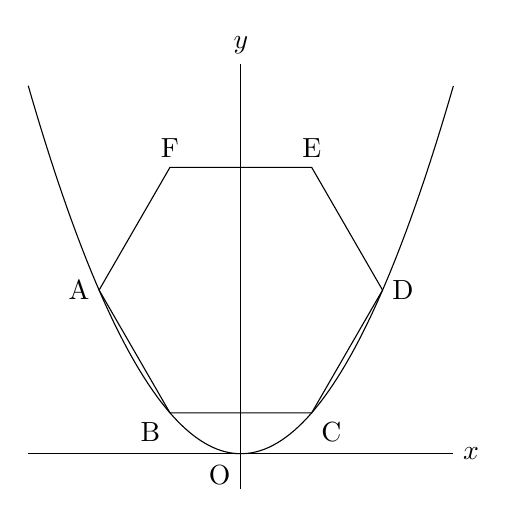
\begin{tikzpicture}[scale=0.9]
    \draw (0,-0.5) -- (0,5.5) node[above] {$y$};
    \draw (-3,0) -- (3,0) node[right] {$x$};
    \node at (-0.3, -0.3) {O};

    \coordinate (A) at (-2, 2.309);
    \coordinate (B) at (-1, 0.577);
    \coordinate (C) at (1, 0.577);
    \coordinate (D) at (2, 2.309);
    \coordinate (E) at (1, 4.041);
    \coordinate (F) at (-1, 4.041);
    
    \draw (A) node[left] {A}-- (B)node[below left] {B} -- (C) node[below right] {C} -- (D) node[right] {D}  -- (E)node[above] {E} -- (F) node[above] {F}-- cycle;

    \draw [domain = -3:3, samples = 100] plot(\x, 0.577*\x*\x);
  \end{tikzpicture}

\item 2直線 $x+y=6$,\ $ax+y=2$の交点をP,\ \ 2直線$x-2y=10$,\ $x+by=-10$の交点をQとする.\\
  2点P,\ \ Qが$x$軸について対称であるとき, $a,\ \ b$の値は,\ \ $a=$\ \fbox{\textcircled{\scriptsize 5} -- ア} ,\ \ $b=$\ \fbox{\textcircled{\scriptsize 5} -- イ}である.
\end{enumerate}

\newpage

\noindent \fbox{\LARGE {\bf 2}}\hspace{10pt} 下の【図1】のように,\ 数直線上の0,\ \ 2,\ \ 4,\ \ 8,\ \ 10,\ \ 12に対応する点をそれぞれO,\ \ A,\ \ B,\ \ C,\ \ D,\ \ Eとする.
\begin{center}
  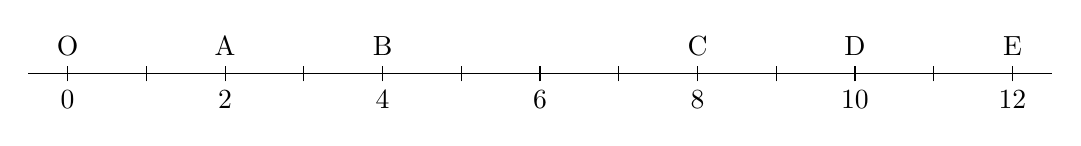
\begin{tikzpicture}[scale=1]
    \draw (-0.5,0)--(12.5,0);
    \draw (0,-0.1)node[below] {0} -- (0,0.1) node[above] {O};
    \draw (1,-0.1) -- (1,0.1);
    \draw (2,-0.1)node[below] {2} -- (2,0.1) node[above] {A};
    \draw (3,-0.1) -- (3,0.1);
    \draw (4,-0.1)node[below] {4} -- (4,0.1) node[above] {B};
    \draw (5,-0.1) -- (5,0.1);
    \draw (6,-0.1) node[below] {6} -- (6,0.1);
    \draw (7,-0.1) -- (7,0.1);
    \draw (8,-0.1) node[below] {8} -- (8,0.1) node[above] {C};
    \draw (9,-0.1) -- (9,0.1);
    \draw (10,-0.1) node[below] {10} -- (10,0.1) node[above] {D};
    \draw (11, -0.1) -- (11, 0.1);
    \draw (12, -0.1) node[below] {12} -- (12, 0.1)node[above] {E};
  \end{tikzpicture}

  【図1】
\end{center}

2点P,\ \ Qは,\ この数直線上を以下の規則にしたがって動く.

\begin{center}
  \begin{tikzpicture}
    \draw[dotted, thick] (-7.5,-1.8) rectangle (8,2.2);
    \draw[dotted, thick] (0,-1.8)--(0,2.2);
    \node at (0,0) {
      \begin{tabular}{p{7cm}p{7cm}}
        $\langle\hspace{-0.1cm} \langle$点P\,$\rangle\hspace{-0.1cm} \rangle$ & $\langle\hspace{-0.1cm} \langle$点Q\,$\rangle\hspace{-0.1cm} \rangle$\\
        \vspace{-0.0cm}
        
        \begin{itemize}
        \item 毎秒2の速さで動く.
        \item Oを出発し,\ O$\to$E$\to$Oの順に動き,\ \ Oで止まる.
        \item 途中のBとDで1秒停止する.
        \item 途中のEで2秒停止する.
        \end{itemize}
                                                                              &\vspace{-0.4cm}
                                                                                
                                                                                \begin{itemize}
                                                                                \item 毎秒3の速さで動く.
                                                                                \item Aを出発し,\ A$\to$E$\to$O$\to$Aの順に動き, Aで止まる.
                                                                                \item 途中のCとAで1秒停止する.
                                                                                \item 途中のEとOで3秒停止する.
                                                                                \end{itemize}
      \end{tabular}
      };
  \end{tikzpicture}
\end{center}

次ページの【図2】は,\ Pの動きを示したグラフである.

2点P,\ \ Qが同時に動き出すとき, 次の\textcircled{\scriptsize 6},\ \textcircled{\scriptsize 7}の\ \fbox{ \hspace{10pt} }\ にあてはまる数を求めなさい.\\
\begin{enumerate}[(1)]
\item P,\ \ Q間の距離が5となる回数は, 全部で\ \fbox{\hspace{5pt}\ \textcircled{\scriptsize 6}\hspace{5pt} }\ 回ある.\\[4cm]
\item P,\ \ Q間の距離がはじめて0になってから,\ \ 2回目に0になるまでに経過する時間は,\ \fbox{\hspace{5pt} \textcircled{\scriptsize 7}\hspace{5pt} }\ 秒である.
\end{enumerate}
\newpage
\begin{center}
  \begin{tikzpicture}[scale = 0.7]
    \draw (0,0) grid (18.5, 12.5);
    \draw[thick] (0,0)--(0,12.5);
    \draw[thick] (0,0)--(18.5,0);

    \draw(-0.1, 2) node[left]{2};
    \draw(-0.1, 4) node[left]{4};
    \draw (-0.1, 6) node[left]{6};
    \draw (-0.1, 8) node[left]{8};
    \draw (-0.1, 10) node[left]{10};
    \draw (-0.1, 12) node[left]{12};

    \draw (5, -0.1) node[below] {5};
    \draw (10, -0.1) node[below] {10};
    \draw (15, -0.1) node[below] {15};
    \node at (18.2,-0.4) {(秒)};

    \node at (-0.3, -0.3) {O};

    \draw[thick] (0,0)--(2,4)--(3,4)--(6,10)--(7,10)--(8,12)--(10,12)--(11,10)--(12,10)--(15,4)--(16,4)--(18,0);
  \end{tikzpicture}

  【図2】
\end{center}
\newpage

\begin{multicols}{2}
  \noindent \fbox{\LARGE {\bf 3}}\hspace{10pt} 点Pを中心として半径6cmの円Pと, 円Qを中心として点Pを通る半径5cmの円Qが, 右の図のように2点A,\ \ Bで交わっている.

  いま, 点Pの周上(ただし, 円Qの内部)に点Cをとり, 点Cをとり, ACの延長と円Qとの交点をDとすると
  , AC\ :\ CD = 2 : 3となった.

  BPの延長と円Pとの交点をEとし, CE,\ \ DPとABとの交点をそれぞれF,\ \ Gとするとき, 次の\textcircled{\scriptsize 8} 〜 \textcircled{\scriptsize 10} の \fbox{ \hspace{10pt} } にあてはまる数を求めなさい.

  \begin{center}
    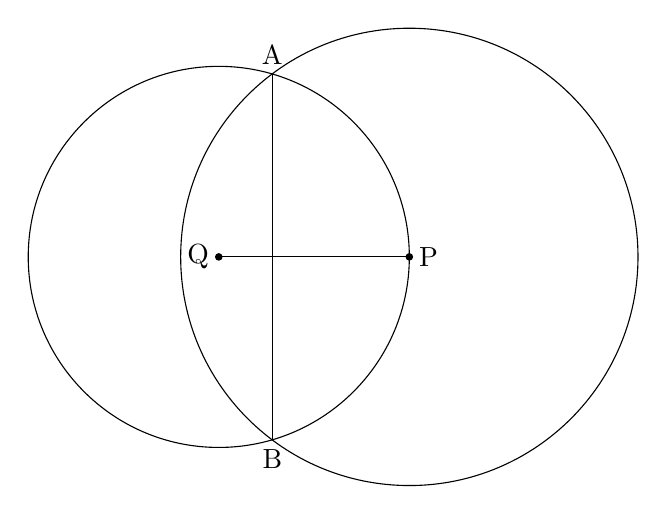
\begin{tikzpicture}[scale=1.21]
      \draw (0,0) circle [radius=2];
      \draw (2, 0) circle[radius=2.4];

      \fill (0,0) node[left] {Q} circle[radius=0.04];
      \fill (2,0) node[right] {P}circle[radius=0.04];

      \draw (0.562, 1.92) node[above] {A} --(0.562,-1.92) node[below] {B};
      \draw (0,0) -- (2,0);
    \end{tikzpicture}
  \end{center}
\end{multicols}

\begin{enumerate}[(1)]
\item 線分ABの長さは \fbox{\hspace{5pt} \textcircled{\scriptsize 8}\hspace{5pt} } cmである.\\[2cm]
\item 線分AGの長さは \fbox{\hspace{5pt} \textcircled{\scriptsize 9}\hspace{5pt} } cmである.\\[2cm]
\item 線分ADの長さは \fbox{\hspace{5pt} \textcircled{\scriptsize 10}\hspace{5pt} } cmである.
\end{enumerate}
\newpage

\begin{multicols}{3}
  \noindent \fbox{\LARGE {\bf 4}}\hspace{10pt} 右の【図3】は, 三角すいの形状の容器の展開図である. $\triangle$OAB, $\triangle$OBC,\ $\triangle$OCAはいずれも直角二等辺三角形で, OA=6cmである.

  【図4】のように, 面ABCを水平にして, この容器いっぱいに水を満たす. このとき, 次の\textcircled{\scriptsize 11} 〜 \textcircled{\scriptsize 13} の \fbox{ \hspace{10pt} } にあてはまる数を求めなさい.

  \begin{center}
    \begin{tikzpicture}
      \coordinate (A) at (-2,0);
      \coordinate (B) at (2,0);
      \coordinate (C) at (0,2);
      \coordinate (O) at (0,0);
      \coordinate (A2) at (0,-2);

      \draw (O)node[below left] {O} -- (A)node[left] {A} -- (C) node[above] {C}-- (B) node[right] {B}-- (A2)node[below] {A}--cycle;
      \draw[dotted] (C)--(O)--(B);
    \end{tikzpicture}

    【図3】
  \end{center}

  \vspace{1.2cm}
  
  \begin{center}
    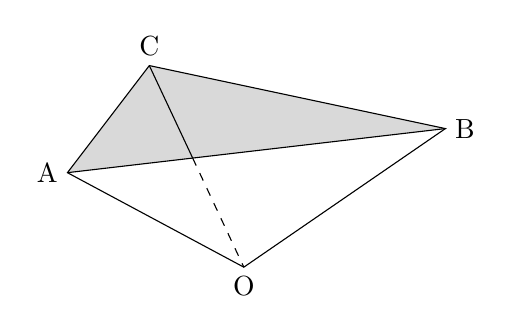
\begin{tikzpicture}[scale = 0.8]
      \coordinate (O) at (0.8,-0.2);
      \coordinate (A) at (-2,1.3);
      \coordinate (B) at (4,2);
      \coordinate (C) at (-0.7, 3);
      \fill[fill=gray!30] (A) node[left] {A}--(B)node[right] {B}--(C)node[above] {C}--cycle;
      \draw (O) node[below] {O}--(A)--(C)--(B)--cycle;
      \draw[name path = C1] (A) -- (B);
      \draw[draw=none, name path = C2] (C)--(O);

      \path[name intersections = {of = C1 and C2}];
      \draw(C)--(intersection-1);
      \draw[dashed] (intersection-1)--(O);
    \end{tikzpicture}

    \vspace{1.1cm}
    
    【図4】
  \end{center}
\end{multicols}

\begin{enumerate}[(1)]
\item 容器に満たされている水の体積は \fbox{\hspace{5pt} \textcircled{\scriptsize 11}\hspace{5pt} } cm${}^{3}$である.\\[2cm]
\item この容器を, 辺BCが水平面と平行である状態を保ちながら, Aを静かに下げて水をこぼしていく.\\[0.1cm]
  容器に残っている水の量が最初の$\displaystyle \frac{1}{4}$になるとき, Oと水面との距離は \fbox{\hspace{5pt} \textcircled{\scriptsize 12}\hspace{5pt} } cmである.\\[2cm]
\item 【図4】の状態に戻して容器いっぱいに水を満たした後, 再び辺BCが水平面と平行である状態を保ちながら, Aを静かに下げて水をこぼしていく.\\
  Oと水面との距離が3cmとなるとき, 水面の面積は \fbox{\hspace{5pt} \textcircled{\scriptsize 13}\hspace{5pt} }cm${}^{2}$である.
\end{enumerate}
\newpage

\noindent \fbox{\LARGE {\bf 5}}\hspace{10pt} 池に住む魚の総数を推測するために, 次のような調査計画を考えた.
\begin{center}
  \begin{tikzpicture}
    \draw (0,0) node[right] {池から魚を無作為に20匹捕獲し, そのすべてに印をつけて池に戻す.};
    \draw (0,-0.4) node[right] {数日後, 同じ池から魚を無作為に20匹捕獲し, その中に印のついた魚が何匹いるのかを調べる.};
    \draw[dotted](-0.1,-0.8) rectangle (15,0.3);
  \end{tikzpicture}
\end{center}

このとき, 次の\textcircled{\scriptsize 14}, \textcircled{\scriptsize 15}の \fbox{ \hspace{10pt} } にあてはまる数,\ \ 式,\ \ 文章等を求めなさい.
\begin{enumerate}[(1)]
\item 池Pにて上記の調査計画を実施したところ, 印のついた魚は8匹捕獲された. この調査結果から推測される魚の総数は \fbox{\textcircled{\scriptsize 14} --  ア } 匹である. どのように推測したのかを \fbox{\textcircled{\scriptsize 14} -- イ} に書きなさい.\\[5cm]
\item 池Qにて上記の調査結果を実施したところ, 印のついた魚は1匹も捕獲されなかった. この調査結果から推測される魚の総数は \fbox{\textcircled{\scriptsize 15} -- ア} 匹である. どのように推測したのかを \fbox{\textcircled{\scriptsize 15} -- イ} に書きなさい.\\

   もし推測しにくい場合は, \fbox{\footnotesize \textcircled{\tiny 15} -- ア} に$\times$を記入し,\ \ どのような調査計画であれば推測しやすくなるか, 新たな調査計画を \fbox{\footnotesize \textcircled{\tiny 15} -- イ} に書きなさい.
\end{enumerate}

\newpage
\thispagestyle{empty}
 
\newpage

\newpage
\thispagestyle{empty}
 
\newpage

\end{document}
